\documentclass[a4paper,11pt]{article}
\usepackage[T1]{fontenc}
\usepackage[utf8]{inputenc}
\usepackage{lmodern}
\usepackage{graphicx}
%\usepackage[french]{babel}
\usepackage{float}

\usepackage[top=2.5cm, bottom=2.5cm, left=2.5cm, right=2.5cm]{geometry}

\usepackage[pdfauthor={Agathe Oddon, Jean-Michel Tozzini},%
pdftitle={LO21 - Rapport de projet},%
pagebackref=true,%
pdftex,%
linkcolor=blue,%
colorlinks]{hyperref}

\begin{document}
\title{LO21 : Rapport de projet\\Calculatrice à notation polonaise inversée}
\author{Agathe Oddon\\Jean-Michel Tozzini}
\date{Printemps 2012}

\maketitle

\section*{Introduction}
Dans le cadre de notre UV LO21, nous devions réaliser la conception puis implémenter en C++ une calculatrice à notation polonaise inversée.

Le rendu final du projet est composé du présent rapport, du code du programme ainsi que de  sa documentation Doxygen.

\tableofcontents

\section{Conception}
\subsection{Diagramme de classes}
	\begin{figure}[H]
		\center
		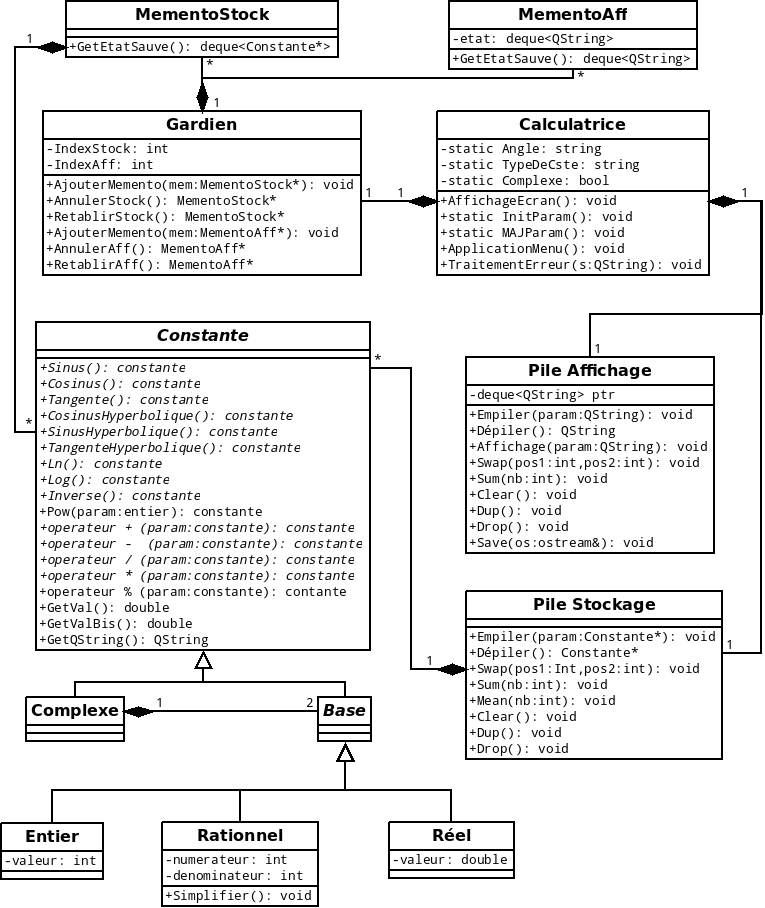
\includegraphics[width=16.7cm]{UMLProjetLO21v3.png}
		\caption{Diagramme de classe de la Calculatrice à notation polonaise inversée}
	\end{figure}
\subsubsection{Types de données}
Nous avons choisi de représenter les données manipulées par la calculatrice comme des objets de trois classes : Entier, Réel, Rationnel, Complexe et Expression. 

La classe complexe est composée de deux objets de type Base, classe abstraite de laquelle dérivent Entier, Réel et Rationnel. Cela permet d'obtenir des complexes composés de deux attributs de types différents.

Les classes Base, Complexe et Expression dérivent de la classe abstraite et exclusive Constante. Ainsi nous empilerons dans la pile de stockage des objets de type Constante.


\subsection{Diagrammes de séquences}
\begin{figure}[H]
	\center
	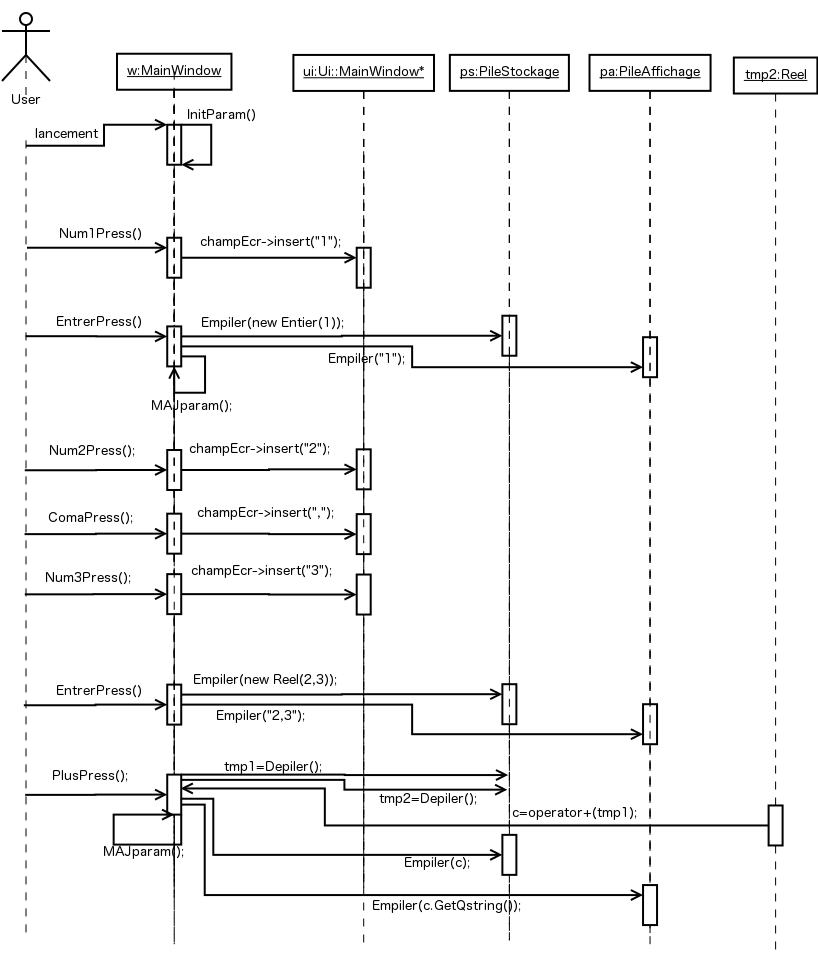
\includegraphics[width=16.7cm]{diag_seq_1.png}
	\caption{Diagramme de séquence décrivant le lancement de la fenêtre, la saisie de "1", "2,3" , l'appui sur le bouton "+" par l'utilisateur, puis l'addition des deux valeurs.}
\end{figure}

\begin{figure}[H]
	\center
	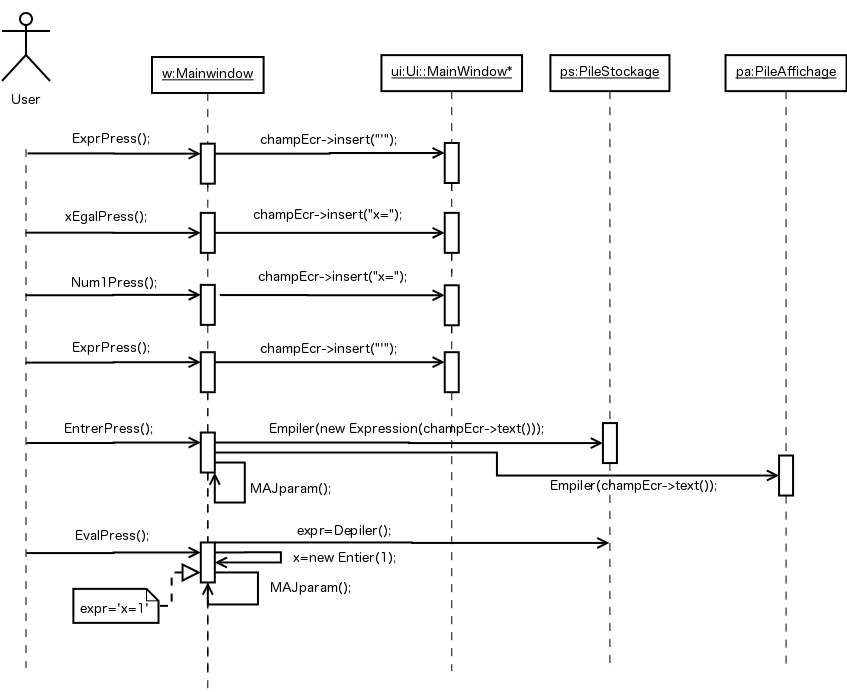
\includegraphics[width=16.7cm]{diag_seq_2.png}
	\caption{Diagramme de séquence décrivant le lancement de la fenêtre, la saisie de 'x=1', puis l'évaluation de l'expression et la sauvegarde de la valeur 1 dans la variable x.}
\end{figure}

\section{Implémentation}
aaaaaaaah
\end{document}
